\documentclass[12pt]{article}

%%%%%%%%%%%%%%%%%%%%%%%%%%%%%%%%%%%
%% Document information  
%%%%%%%%%%%%%%%%%%%%%%%%%%%%%%%%%%%

\title{Declarative Modeling of Proton Exchange Membrane Fuel Cells \\ for System Design}
\author{Kevin L. Davies}
\newcommand{\subtitle}{Ph.D. Research Summary}
\newcommand{\keywords}{proton exchange membrane fuel cell;system design;declarative;model;Modelica;electrochemistry;mass transport;momentum transport;heat transport;advection;diffusion}        

%%%%%%%%%%%%%%%%%%%%%%%%%%%%%%%%%%%
%% Load packages and files  
%%%%%%%%%%%%%%%%%%%%%%%%%%%%%%%%%%%

% Load packages.
\usepackage{../Templates/davies-math} % Load custom macros for math.
\usepackage{../Templates/davies} % Load basic packages and macros.
% \usepackage{davies-dissertation} % Custom settings
% \usepackage{../Templates/davies-hyperref} % Create hyperlinks.
\usepackage[glshyper]{../Templates/davies-glossaries} % Create custom macros based on the glossaries package.
\usepackage[margin=1in]{geometry} % Adjust the margins.

% Load the glossary entries from external files.
\loadglsentries{../Nomenclature/main}
% \loadglsentries{../Nomenclature/stdabbr}
\loadglsentries{../Nomenclature/acronyms}
% \loadglsentries{../Nomenclature/symbols}
% \loadglsentries{../Nomenclature/accents}
% \loadglsentries{../Nomenclature/underscores}
% \loadglsentries{../Nomenclature/superscripts}
% \loadglsentries{../Nomenclature/subscripts}
% \loadglsentries{../Nomenclature/chemicals}

% Set up the references.
%\bibfiles{../../References/primary} 
                  
% Specify the directory where figure images are located.
% Note: This can be used to build the document with alternate images.
\graphicspath{{Figures/}}
\pdfminorversion=5 % Support PDF version 1.5 (otherwise, 1.4).

% Suppress some of the underfull/overfull warnings.
\hbadness=10000 % Underfull \hbox.  (Occurring due to some of the URLs in the references section.)
\hfuzz=10000pt % Overfull \hbox.  (Occurring in the list of notation.)

% Redefine the maketitle command to:
%   1. Remove the date field and the space associated with it.
%   2. Make the title smaller.
%   3. Add a subtitle. 
\makeatletter
\renewcommand{\@maketitle}{
  \newpage                
  %\null
  %\vskip 2em%
  \begin{center}%
    \let \footnote \thanks
    %{\LARGE \@title \par}%
    {\large \@title \par}%
    \vskip 1em%
    {%\large
    \lineskip .5em%
    \begin{tabular}[t]{c}%
    \subtitle
    \end{tabular}\par}
    \vskip 1em%
    {%\large
    \lineskip .5em%
    \begin{tabular}[t]{c}%
    \@author
    \end{tabular}\par}
    \vskip 1em%
    %{\large \@date}%
    \end{center}
    \par
    \vskip 1.5em}
\makeatother

%%%%%%%%%%%%%%%%%%%%%%%%%%%%%%%%%%%
%% Document
%%%%%%%%%%%%%%%%%%%%%%%%%%%%%%%%%%%

\begin{document}

\maketitle{\title}
\thispagestyle{empty}

The goal of this research is to realize the advantages of declarative modeling for complex physical systems that involve both advection and diffusion to varying degrees in multiple domains.  This occurs, for example, in chemical devices such as fuel cells.  The declarative or equation-based modeling approach can provide computational advantages and is compatible with physics-based, object-oriented representations.  However, there is no generally accepted method of representing coupled advection and diffusion in a declarative modeling framework.  

This work develops, justifies, and implements a new upstream discretization scheme for mixed advective and diffusive flows that is well-suited for declarative models.  The discretization scheme yields a gradual transition from pure diffusion to pure advection without switching events or nonlinear systems of equations.  Transport equations are established in a manner that ensures the conservation of material, momentum, and energy at each interface and in each control volume.  The approach is multi-dimensional and resolved down to the species level, with conservation equations for each species in each phase.  The framework is applicable to solids, liquids, gases, and charged particles.  Interactions among species are described as exchange processes which are diffusive if the interaction is inert or advective if it involves chemical reactions or phase change.

The equations are implemented in a highly modular and reconfigurable manner using the Modelica language.  A wide range of examples are demonstrated---from basic models of electrical conduction and evaporation to a comprehensive model of a \n{PEMFC}.  Several versions of the \n{PEMFC} model are simulated under various conditions including polarization tests and a cyclical electrical load.  The model is shown to describe processes such as electro-osmotic drag and liquid pore saturation.  It can be scaled in complexity from \num{4000} to \num{32000} equations, resulting in a simulation times from 0.2 to \SI{19}{s} depending on the level of detail.  The most complex example is a seven-layer cell with six segments along the length of the channel.  The model library is thoroughly documented and made available as a free, open-source software package.


% Use the first occurrence version of all of the abbreviations after the summary.
\glsresetall


\begin{figure}[htbp!]
\centering
\subfloat[Test configuration]{
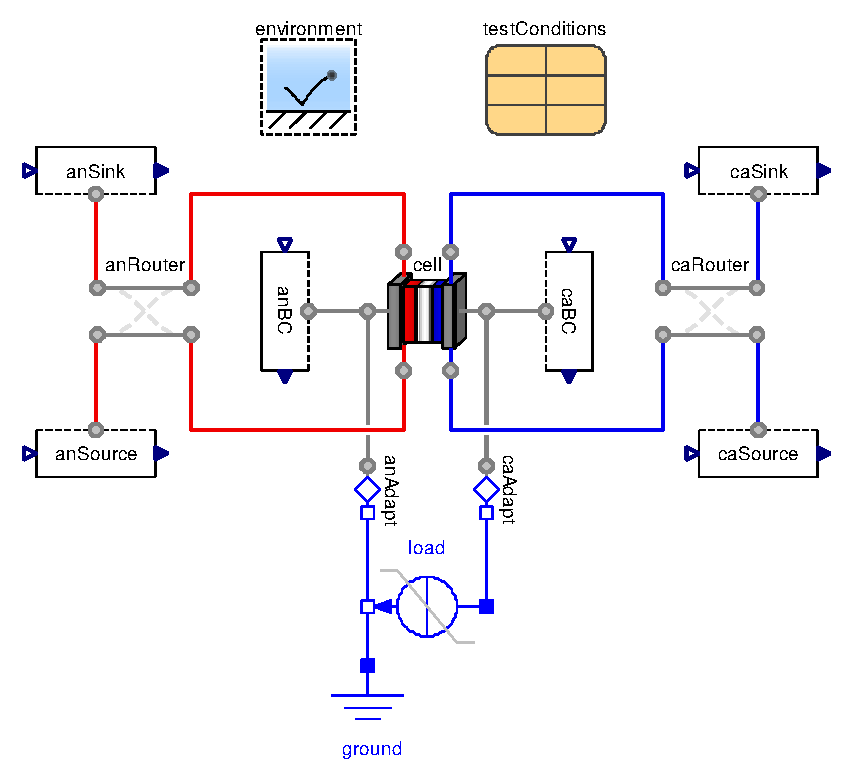
\includegraphics[width=0.42\textwidth]{4-TestStandD}%
}\quad
\subfloat[Layers of the cell]{
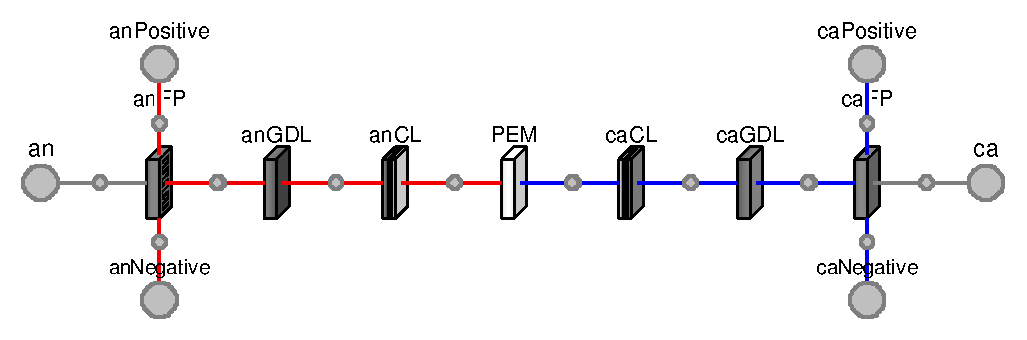
\includegraphics[width=0.52\textwidth]{4-CellD}%
}
\caption{Diagrams showing the declarative, object-oriented nature of the PEMFC model}%
\end{figure}

\end{document}